\documentclass[fontsize=11pt,]{article}
\usepackage{graphicx}
\usepackage{pdfpages}

% \parindent10pt
\raggedright

%Geometry Package
\usepackage[
    paper=a4paper,
    top=45mm,
    bottom=15mm,
    right=15mm,
    left=57mm,
    % showframe,  %change opacity to see frame
]{geometry}

% Background package
\usepackage[
    pages=some,
    scale=1,
    color=black,
    opacity=1.0,  % change opacity to see position of frame
    angle=0,
]{background}
\backgroundsetup{contents={
\includegraphics[width=\paperwidth,
        height=\paperheight]{au-dbs-letterhead.pdf}}}

% ----------------------------------------------------
% Letter
\begin{document}
\vspace*{-3\baselineskip}
\BgThispage
\hfill \today\\
\vspace{2mm}
\textbf{Re: Tissue Loan Request}\\
\vspace{2mm}

Dear Dr. Jerry Johnson, \\

\vspace{2mm}

I am writing to request tissue samples from the following specimens in
The University of Texas at El Paso Biodiversity Collection:

% \vspace{5mm}
% \vspace{\baselineskip}

\vspace*{-2mm}

\begin{table}[h]
\begin{tabular}{ll}

    UTEP 18705 Anaxyrus woodhousii  &  UTEP 21286 Anaxyrus speciosus \\
    UTEP 19941 Anaxyrus woodhousii  &  UTEP 21724 Anaxyrus speciosus \\
    UTEP 19943 Anaxyrus woodhousii  &  UTEP 21881 Anaxyrus cognatus \\
    UTEP 19947 Anaxyrus terrestris  &  UTEP 21884 Anaxyrus speciosus \\
    UTEP 20105 Anaxyrus woodhousii  &  UTEP 21885 Anaxyrus speciosus \\
    UTEP 20921 Anaxyrus woodhousii  &  UTEP 21886 Anaxyrus woodhousii \\
    UTEP 21284 Anaxyrus debilis  &  \\

\end{tabular}
\end{table}

\vspace*{-2mm}

These tissues will be used to obtain RADseq data for a phylogeographic study of
North American toads in the genus \textit{Anaxyrus}.
The samples we are requesting will make up a broader sample of 109 tissues from 
other institutions, including 33 from the Auburn Museum of Natural History (see attached map)
The aim of this study is to infer the relationships among species and
populations in this genus using a large genome-wide data set.
Previous estimates of the phylogeny of \textit{Anaxyrus} 
from a small number of mitochondrial and nuclear loci have been inconsistent  
which suggests these limited data may not be sufficient.
Furthermore, these data sets are not adequate for detecting historic
admixture which may have been an important process in the evolution of
\textit{Anaxyrus}.
Numerous instances of natural hybridization have been reported in the literature
and breeding crosses have demonstrated reproductive compatibility between many
species pairs that have overlapping or adjoining distributions. \\

\vspace{2mm}

This study will complement another ongoing study examining
introgression at a hybrid zone between the American toad and Southern toad in
central Alabama.
We have collected 202 individuals from this hybrid zone and deposited 
them into the Auburn University Museum of Natural History.
We will obtain RADseq data from these individuals to quantify the extent of
introgression across this hybrid zone and test for variation in the rate of
introgression across the genome due to selection.
Inference of species relationships, relative timing of divergence, and historic
admixture using the samples that we are requesting will provide important
context for this hybrid zone study and unprecedented detail on the evolutionary
history of this prominent group of vertebrates in North America.

\vspace{2mm}

Our lab has a significant amount of experience collecting RADseq data for phylogeographic
studies. Our lab is equipped to collect these data and we have access to great 
computation resources for conducting analyses. This project will be funded by an 
NSF grant awarded in 2017. We will prepare libraries from the samples immediately   
and add them to already prepared libraries for sequencing before the end of the
current semester. Analyses will be performed during the Summer and upcoming Fall 
semester. We plan to complete this project and publish the results by the end of 
this year.

\vspace{2mm}

Sincerely,\\

\vspace{2mm}
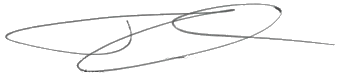
\includegraphics[height=2.0\baselineskip]{jamie_signature.png}\\

Jamie Oaks\\
Assistant Professor and Curator \\
Museum of Natural History\\
101 Rouse Life Sciences Building\\
Auburn University\\
Auburn, Alabama 36849, USA

\end{document}